%%%%%%%%%%%%%%%%%%%%%%%%%%%%%%%%%%%%%%%%%
% baposter Landscape Poster
% LaTeX Template
% Version 1.0 (11/06/13)
%
% baposter Class Created by:
% Brian Amberg (baposter@brian-amberg.de)
%
% This template has been downloaded from:
% http://www.LaTeXTemplates.com
%
% License:
% CC BY-NC-SA 3.0 (http://creativecommons.org/licenses/by-nc-sa/3.0/)
%
%%%%%%%%%%%%%%%%%%%%%%%%%%%%%%%%%%%%%%%%%

%----------------------------------------------------------------------------------------
%	PACKAGES AND OTHER DOCUMENT CONFIGURATIONS
%----------------------------------------------------------------------------------------

\documentclass[landscape,a0paper,fontscale=0.375]{baposter} % Adjust the font scale/size here (fontscale=0.285)

\usepackage{graphicx} % Required for including images
\graphicspath{{figures/}} % Directory in which figures are stored

\usepackage{amsmath} % For typesetting math
\usepackage{amssymb} % Adds new symbols to be used in math mode

\usepackage{booktabs} % Top and bottom rules for tables
\usepackage{enumitem} % Used to reduce itemize/enumerate spacing
\usepackage{palatino} % Use the Palatino font
\usepackage[font=small,labelfont=bf]{caption} % Required for specifying captions to tables and figures

\usepackage{multicol} % Required for multiple columns
\setlength{\columnsep}{1.5em} % Slightly increase the space between columns
\setlength{\columnseprule}{0mm} % No horizontal rule between columns

\usepackage{xcolor} % color in RGB

\usepackage{tikz} % Required for flow chart
\usetikzlibrary{shapes,arrows} % Tikz libraries required for the flow chart in the template

%\usepackage{etex}			%%%%% bib setup from our main
%\usepackage{etoolbox}
%\usepackage{keyval}
%\usepackage{ifthen}
%\usepackage{url}
%\usepackage{csquotes}
%\usepackage[backend=biber, url=true, doi=true, style=numeric, sorting=none]{biblatex}

\newcommand{\compresslist}{ % Define a command to reduce spacing within itemize/enumerate environments, this is used right after \begin{itemize} or \begin{enumerate}
\setlength{\itemsep}{1pt}
\setlength{\parskip}{0pt}
\setlength{\parsep}{0pt}
}

%\definecolor{lightblue}{RGB}{33,26,82} % Defines the color used for content box headers
\definecolor{lightblue}{rgb}{0.145,0.6666,1} % Defines the color used for content box headers
\definecolor{aaublue}{rgb}{0.1294117647,0.1019607843,0.3215686275}  %<--define aaublue

\begin{document}

\begin{poster}
{
headerborder=closed, % Adds a border around the header of content boxes
colspacing=1em, % Column spacing
bgColorOne=white, % Background color for the gradient on the left side of the poster
bgColorTwo=white, % Background color for the gradient on the right side of the poster
borderColor=lightblue, % Border color
headerColorOne=aaublue, % Background color for the header in the content boxes (left side)
headerColorTwo=lightblue, % Background color for the header in the content boxes (right side)
headerFontColor=white, % Text color for the header text in the content boxes
boxColorOne=white, % Background color of the content boxes
textborder=roundedleft, % Format of the border around content boxes, can be: none, bars, coils, triangles, rectangle, rounded, roundedsmall, roundedright or faded
eyecatcher=true, % Set to false for ignoring the left logo in the title and move the title left
headerheight=0.1\textheight, % Height of the header
headershape=roundedright, % Specify the rounded corner in the content box headers, can be: rectangle, small-rounded, roundedright, roundedleft or rounded
headerfont=\Large\bf\textsc, % Large, bold and sans serif font in the headers of content boxes
%textfont={\setlength{\parindent}{1.5em}}, % Uncomment for paragraph indentation
linewidth=2pt % Width of the border lines around content boxes
}
%----------------------------------------------------------------------------------------
%	TITLE SECTION 
%----------------------------------------------------------------------------------------
%
{
\includegraphics[height=2.7em]{group7404.png}} % First university/lab logo on the left
{\bf \fontsize{1.5cm}{1.5cm} THE \hspace{3pt} EFFECT \hspace{3pt} OF \hspace{3pt} LIMB \hspace{3pt} POSITION \hspace{3pt} ON \hspace{3pt} MYOELECTRIC \hspace{3pt} PROSTHETIC \hspace{3pt} CONTROL\\ \vspace{0.2em} USING \hspace{3pt} LINEAR \hspace{3pt} REGRESSION \vspace{0.5em}} % Poster title %The effect of limb position on myoelectric prosthetic control using linear regression 
{\ \textit{Irene Uriarte, Martin Garenfeld, Oliver Damsgaard, Simon Bruun.} \hspace{1pt} Aalborg University, School of Medicine and Health \vspace{0.05em}} % Author names and institution
{
\includegraphics[height=7em]{AAU_LOGO_RGB_UK.png}} % Second university/lab logo on the right

%----------------------------------------------------------------------------------------
%	INTRODUCTION
%----------------------------------------------------------------------------------------

\headerbox{Introduction}{name=introduction,column=0,row=0}{
	
	%The development of EMG controlled prosthetics have advanced greatly in recent years. More complex prosthetics are demanded and more advanced control mothods has been developed. Most control methods so far has utilized pattern recognition which only enables control of one degree of freedom at a time. Most studies have conducted tests in only one limb position, not considering the limb position effect on EMG signals. \cite{Fougner2011} This study aims to overcome the limb position effect by combining EMG with inertial information in the training sessions of the regressor to obtain simultaneous and proportional control of EMG prosthesis.
	Electromyography (EMG) is widely used for controlling functional prosthetics. However, EMG signals for the same movements change with variations in limb position and lowers the accuracy in control schemes \cite{Fougner2011}. Most previous studies have utilized classification for pattern recognition when changing limb position, with a negative effect in performance. Linear regression is a newer method in control of myoelectric prosthetics, which has proven to yield robust simultaneous and proportional control \cite{hahne2014}. Only the RMS feature was previously tested in variations of limb positions in regression-based control \cite{Hwang2017}. This study investigated the effect of limb position in a linear regression-based control scheme, when using the commonly used Mean Absolute Value (MAV) and Logarithmic Variance (LogVar) feature, where the latter has shown linear properties \cite{hahne2014}.
}

%----------------------------------------------------------------------------------------
%	OBJECTIVES   bottomaligned=objectives
%----------------------------------------------------------------------------------------

\headerbox{Aim}{name=aim,column=1,row=0}{

The aim for this project are expressed in the following two hypotheses:

%hypotheses
\begin{itemize}
	\item Simultaneous and proportional control of two DOF's of the wrist in different limb positions, can be achieve trough the use of linear regression as control system. 
	\item Combining ssurface EMG and IMU's can minimize the limb position effect when using regression as control system. 
\end{itemize}

\vspace{0.3em} % When there are two boxes, some whitespace may need to be added if the one on the right has more content
}

%----------------------------------------------------------------------------------------
%	RESULTS 1	Online training results
%----------------------------------------------------------------------------------------

\headerbox{Online Results}{name=results,column=2,span=2,row=0}{

Results for the online test of regressor accuracy and control. The test is performed in a modified Fitts' Law test of reaching targets. The score is calculated as the relation between time and number of targets reached.
\begin{multicols}{2}
	 
\vspace{1em}

\begin{center}
	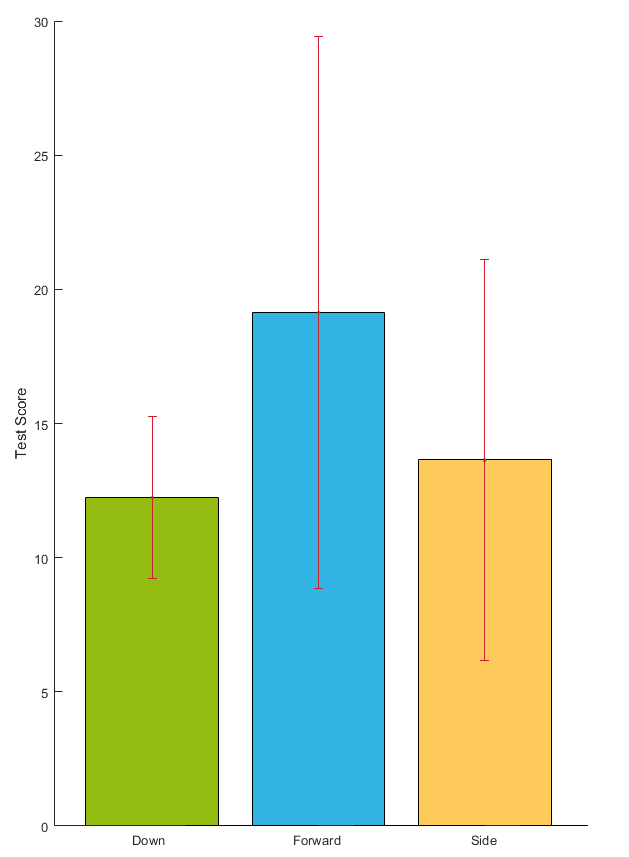
\includegraphics[width=0.3\linewidth]{TestScore}
	\captionof{figure}{The mean test score among four subjects when using regressors trained with Log-Var excluding IMU information}
\end{center}


\begin{center}
	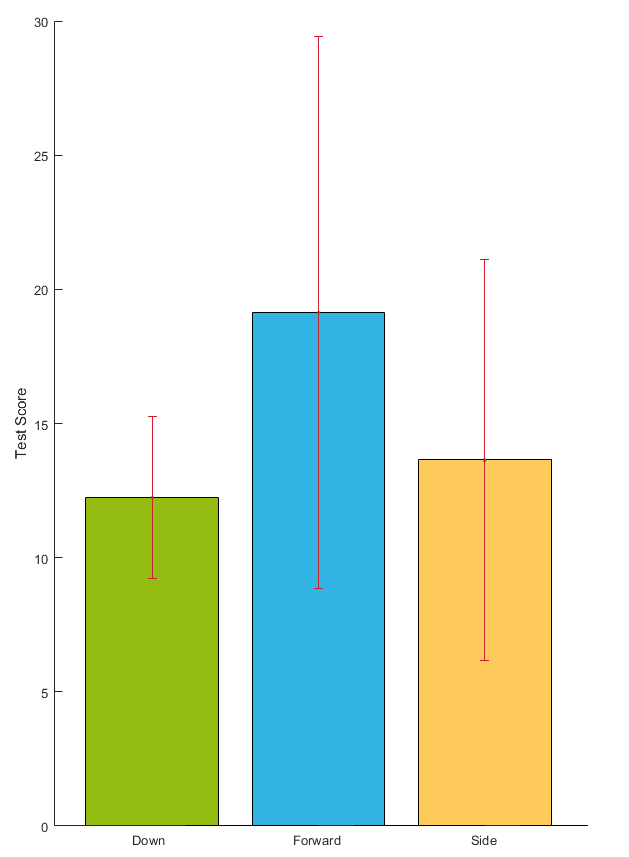
\includegraphics[width=0.3\linewidth]{TestScore}
	\captionof{figure}{The mean test score among four subjects when using regressors trained with Log-Var excluding IMU information}
\end{center}

*** text ***

\end{multicols}

placeholder text. placeholder text. placeholder text. placeholder text. placeholder text. placeholder text. placeholder text. placeholder text. placeholder text. placeholder text. placeholder text. placeholder text. placeholder text. placeholder text. placeholder text. placeholder text. placeholder text. placeholder text. placeholder text. placeholder text. placeholder text. placeholder text. placeholder text. placeholder text. placeholder text. placeholder text. placeholder text. placeholder text. placeholder text. placeholder text. placeholder text. placeholder text. placeholder text. placeholder text. placeholder text. placeholder text. placeholder text. placeholder text. placeholder text. placeholder text. placeholder text. placeholder text. 

%%------------------------------------------------
%
%\begin{multicols}{2}
%
%\begin{center}
%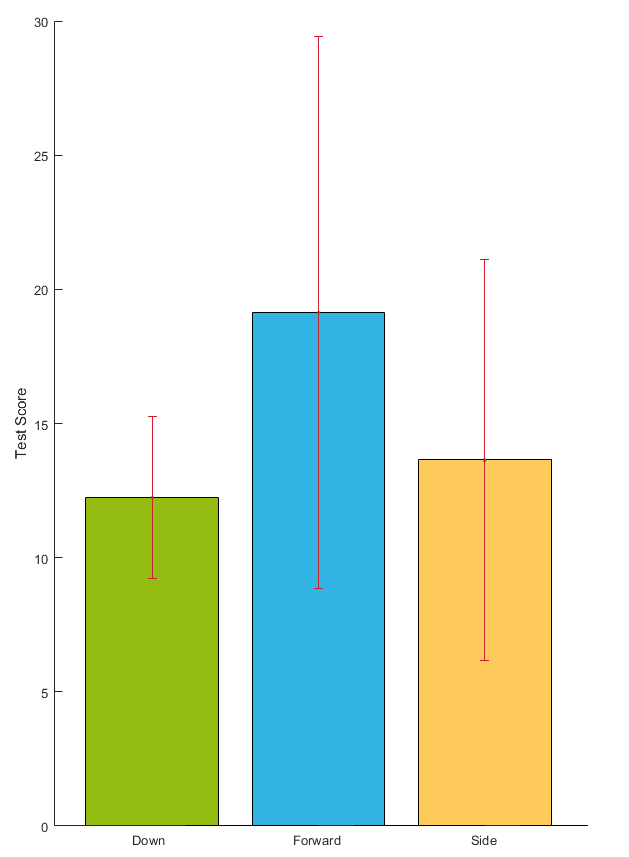
\includegraphics[width=0.2\linewidth]{TestScore}
%\captionof{figure}{The mean test score among four subjects when using regressors trained with Log-Var including IMU information}
%\end{center}
% 
%text?
%\end{multicols}
}

%----------------------------------------------------------------------------------------
%	REFERENCES
%----------------------------------------------------------------------------------------

\headerbox{References}{name=references,column=1,span=2,above=bottom}{

\renewcommand{\section}[2]{\vskip 0.05em} % Get rid of the default "References" section title
\nocite{*} % Insert publications even if they are not cited in the poster
\small{ % Reduce the font size in this block
\bibliographystyle{unsrt}
\bibliography{sample} %%% MANUALLY ADD SOURCES FROM THE MAIN.BIB TO THE SAMPLE.BIB !!!
}}

%----------------------------------------------------------------------------------------
%	FUTURE RESEARCH
%----------------------------------------------------------------------------------------
%
%\headerbox{Future Research}{name=futureresearch,column=1,span=2,aligned=references,above=bottom}{ % This block is as tall as the references block
%
%\begin{multicols}{2}
%Integer sed lectus vel mauris euismod suscipit. Praesent a est a est ultricies pellentesque. Donec tincidunt, nunc in feugiat varius, lectus lectus auctor lorem, egestas molestie risus erat ut nibh.
%
%Maecenas viverra ligula a risus blandit vel tincidunt est adipiscing. Suspendisse mollis iaculis sem, in \emph{imperdiet} orci porta vitae. Quisque id dui sed ante sollicitudin sagittis.
%\end{multicols}
%}

%----------------------------------------------------------------------------------------
%	CONTACT INFORMATION
%----------------------------------------------------------------------------------------

\headerbox{Contact Information}{name=contact,column=3,aligned=references,above=bottom}{ % This block is as tall as the references block

\begin{description}\compresslist
\item[Web] www.smh.aau.dk
\item[Email] 17gr7404@hst.aau.dk
%\item[Phone] +1 (000) 111 1111
\end{description}
}

%----------------------------------------------------------------------------------------
%	CONCLUSION
%----------------------------------------------------------------------------------------

\headerbox{Conclusion}{name=conclusion,column=2,span=2,row=0,below=results,above=references}{

\begin{multicols}{2}

\tikzstyle{decision} = [diamond, draw, fill=blue!20, text width=4.5em, text badly centered, node distance=2cm, inner sep=0pt]
\tikzstyle{block} = [rectangle, draw, fill=blue!20, text width=5em, text centered, rounded corners, minimum height=4em]
\tikzstyle{line} = [draw, -latex']
\tikzstyle{cloud} = [draw, ellipse, fill=red!20, node distance=3cm, minimum height=2em]

\begin{tikzpicture}[node distance = 2cm, auto]
\node [block] (init) {Initialize Model};
\node [cloud, left of=init] (Start) {Start};
\node [cloud, right of=init] (Start2) {Start Two};
\node [block, below of=init] (init2) {Initialize Two};
\node [decision, below of=init2] (End) {End};
\path [line] (init) -- (init2);
\path [line] (init2) -- (End);
\path [line, dashed] (Start) -- (init);
\path [line, dashed] (Start2) -- (init);
\path [line, dashed] (Start2) |- (init2);
\end{tikzpicture}

%------------------------------------------------

\begin{itemize}\compresslist
\item Pellentesque eget orci eros. Fusce ultricies, tellus et pellentesque fringilla, ante massa luctus libero, quis tristique purus urna nec nibh. Phasellus fermentum rutrum elementum. Nam quis justo lectus.
\item Vestibulum sem ante, hendrerit a gravida ac, blandit quis magna.
\item Donec sem metus, facilisis at condimentum eget, vehicula ut massa. Morbi consequat, diam sed convallis tincidunt, arcu nunc.
\item Nunc at convallis urna. isus ante. Pellentesque condimentum dui. Etiam sagittis purus non tellus tempor volutpat. Donec et dui non massa tristique adipiscing.
\end{itemize}

\end{multicols}
}

%----------------------------------------------------------------------------------------
%	MATERIALS AND METHODS
%----------------------------------------------------------------------------------------

\headerbox{Methods}{name=method,column=0,below=introduction,bottomaligned=references}{ % This block's bottom aligns with the bottom of the conclusion block

Surface EMG data was collected from four able-bodied subjects. Subjects were instructed to performed four different hand gestures. This study only focus on two DOF, which are, flexion and extension, radial and ulnar deviation of the wrist. sEMG signals were recorded with Myo armband, positioned on the right forearm of the subjects while standing.

The sEMG was recorded by eight channels in a frequency range 0-200Hz. IMU data was recorded using the buildt in accelerometer in the Myo armband. Filtering were done through a second-order Butterworth high-pass filter ($f_c$=10Hz). 

Features are extracted using a sliding-window of 40 samples with an overlapping of the 50\%. Two time domain features are extracted; Mean absolute value (MAV) and logarithmic variance (LogVar). MAV represent the amplitud of the signal. It is defined as the average of the absolute values of the sEMG signal:
\vspace{-0.2cm}
\begin{equation}
MAV = \frac{1}{N}\sum\limits_{i=1}^N|x_i|
\end{equation} \vspace{-0.1cm}

where N is the length of the signal, and $x_i$ is the signal of $i$ samples.
LogVar is a nonlinear transformation of the variance %applied to %linealidad
\vspace{-0.2cm}
\begin{equation} \label{eq:logvar}
log(\sigma^2) = log(\frac{\sum\limits_{i=1}^N(x_i - \mu)^2}{N})
\end{equation}\vspace{-0.1cm}

where $N$ is the length of the signal, $x_i$ is the $i^th$ sample of the signal and $\mu$ is the mean.
%PCA is applied to qualitatively determine the separability of the feature data. Data is evaluated for differncies in feature data clusters and significant outliers. If the feature clusters are distinguishable from each other and have no significant outliers, the data is of high quality and will be used to train the regressors. Only the first three principal components identified through PCA will be used to train the regressors.
The regressors are implemented through simple linear regression:
\vspace{-0.1cm}
\begin{equation} \label{eq:simpleLinearRegression}
Y = \alpha + \beta X + \epsilon
\end{equation} \vspace{-0.1cm}

where $Y$ is the dependent variable or response, $X$ is the independent variable or the predictor, $\beta$ is the regression coefficient or the slope, and $\alpha$ is the Y intercept (predicted value of $Y$ at $X = 0$),  $\epsilon$ is the error.
The regressor accuracy of control is tested qualitatively through superimposition of the output of the regressors build for each feature onto the actual data for the intensities of the movements. The regressor accuracy is quantitatively tested through a target reaching task measuring time to reach 16 targets. The performance (time per reached target) of the online test was compared between the different limb positions of the same feature and between all limb positions of the two features through statistical analysis. \vspace{0.5cm}
}

%----------------------------------------------------------------------------------------
%	RESULTS 2 Offline training results
%----------------------------------------------------------------------------------------

\headerbox{Offline Results}{name=results2,column=1,below=aim,bottomaligned=conclusion}{ % This block's bottom aligns with the bottom of the conclusion block

Results of the superimposition of the regressor outputs on the estimated data.
\begin{center}
	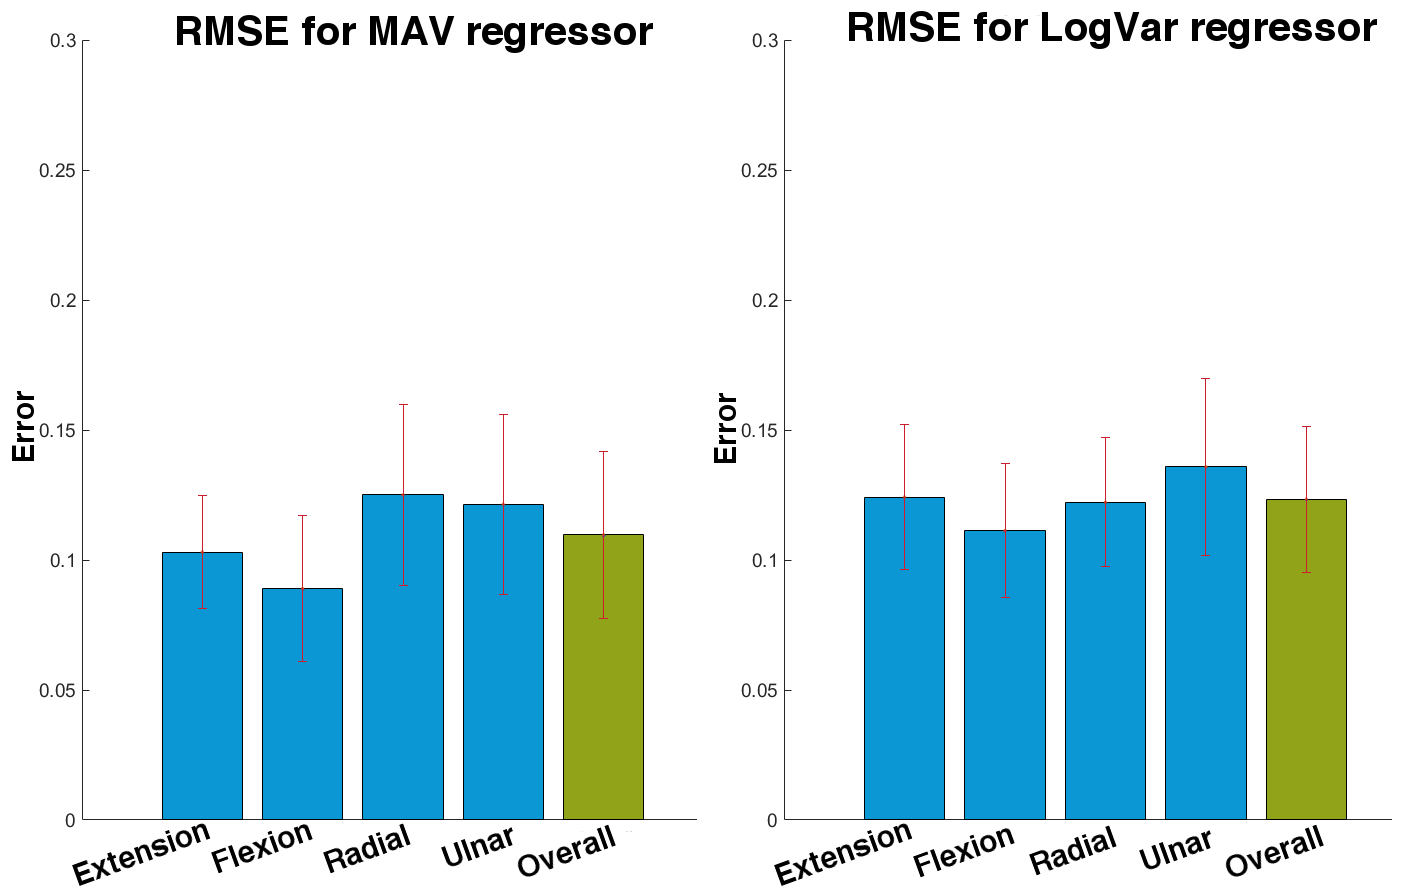
\includegraphics[width=0.9\linewidth]{gimmeThemRMSEBars}
	\captionof{figure}{DATA}
\end{center}

The results for the offline test of accuracy of the regressors of both test and training data. This test determines if the training of the regressors have over- or under-fitted to the training data. 

\begin{center}
\begin{tabular}{l l l}
\toprule
\textbf{Feature} & \textbf{Overall mean error} & \textbf{Highest mean error}\\
\midrule
MAV & 0.0943 $\pm 0.0290$ & 0.1088 $\pm 0.0366$ \\
Log-Var & 0.1107 $\pm 0.0298$ & 0.1216 $\pm 0.0402$ \\
\bottomrule
\end{tabular}
\captionof{table}{RMSE of training data}
\end{center}

*** maybe put some text here to devide the tables ***

\begin{center}
\begin{tabular}{l l l}
\toprule
\textbf{Feature} & \textbf{Overall mean error} & \textbf{Highest mean error}\\
\midrule
MAV & ??? $\pm ???$ & ??? $\pm ???$ \\
Log-Var & ??? $\pm ???$ & ??? $\pm ???$ \\
\bottomrule
\end{tabular}
\captionof{table}{RMSE of test data}
\end{center}
}

%----------------------------------------------------------------------------------------

\end{poster}

\end{document}